%% ============================================================
%%  Aevora — A Multi-Platform WireGuard-Based VPN System
%%  Computer Networks Mini-Project Report
%%  SSN College of Engineering, Chennai  |  AY 2026–2027
%% ============================================================
\documentclass[12pt,a4paper]{report}

\usepackage[T1]{fontenc}
\usepackage[utf8]{inputenc}
\usepackage[a4paper, top=25mm, bottom=25mm, left=30mm, right=20mm]{geometry}
\usepackage{microtype}
\usepackage{setspace}
\usepackage{parskip}
\usepackage{titlesec}
\usepackage{fancyhdr}
\usepackage{booktabs}
\usepackage{longtable}
\usepackage{array}
\usepackage{tabularx}
\usepackage{enumitem}
\usepackage{listings}
\usepackage{xcolor}
\usepackage{amsmath}
\usepackage{amssymb}
\usepackage[hidelinks, colorlinks=true, linkcolor=black, citecolor=blue!60!black, urlcolor=blue!60!black]{hyperref}
\usepackage[backend=bibtex, style=ieee, sorting=none]{biblatex}
\addbibresource{aevora-report.bib}
\usepackage{tikz}
\usetikzlibrary{arrows.meta, shapes.geometric, positioning, fit, backgrounds, calc}
\usepackage{pgfplots}
\pgfplotsset{compat=1.18}
\usepackage{caption}
\usepackage{float}
\usepackage{tocloft}

\onehalfspacing
\setlength{\parskip}{4pt}

%% Headings
\titleformat{\chapter}[block]{\normalfont\Large\bfseries}{CHAPTER \thechapter}{1em}{\uppercase}
\titlespacing*{\chapter}{0pt}{-10pt}{14pt}
\titleformat{\section}{\normalfont\large\bfseries}{\thesection}{1em}{}
\titleformat{\subsection}{\normalfont\normalsize\bfseries}{\thesubsection}{1em}{}

%% Header/Footer
\pagestyle{fancy}\fancyhf{}
\renewcommand{\headrulewidth}{0.4pt}\renewcommand{\footrulewidth}{0.4pt}
\fancyhead[L]{\small\textit{Aevora: A Multi-Platform WireGuard-Based VPN System}}
\fancyhead[R]{\small\textit{SSN College of Engineering}}
\fancyfoot[C]{\small\thepage}

%% Code
\definecolor{codebg}{rgb}{0.97,0.97,0.97}
\definecolor{codeframe}{rgb}{0.82,0.82,0.82}
\definecolor{codecomment}{rgb}{0.25,0.50,0.25}
\definecolor{codekw}{rgb}{0.1,0.1,0.7}
\lstset{
  backgroundcolor=\color{codebg}, frame=single, framesep=3pt, rulecolor=\color{codeframe},
  basicstyle=\ttfamily\small, keywordstyle=\color{codekw}\bfseries,
  commentstyle=\color{codecomment}\itshape, stringstyle=\color{red!60!black},
  breaklines=true, showstringspaces=false,
  numbers=left, numberstyle=\tiny\color{gray}, xleftmargin=6mm
}

%% TikZ styles
\tikzset{
  wbox/.style={rectangle,rounded corners=3pt,draw=gray!60,fill=gray!8,text width=3.0cm,align=center,minimum height=0.9cm,font=\small},
  bbox/.style={rectangle,rounded corners=3pt,draw=blue!60,fill=blue!8,text width=3.0cm,align=center,minimum height=0.9cm,font=\small},
  gbox/.style={rectangle,rounded corners=3pt,draw=green!60!black,fill=green!8,text width=3.0cm,align=center,minimum height=0.9cm,font=\small},
  rbox/.style={rectangle,rounded corners=3pt,draw=red!60,fill=red!8,text width=3.0cm,align=center,minimum height=0.9cm,font=\small},
  obox/.style={rectangle,rounded corners=3pt,draw=orange!70!black,fill=orange!8,text width=3.0cm,align=center,minimum height=0.9cm,font=\small},
  pbox/.style={rectangle,rounded corners=3pt,draw=purple!60,fill=purple!8,text width=3.0cm,align=center,minimum height=0.9cm,font=\small},
  tbox/.style={rectangle,rounded corners=3pt,draw=teal!60,fill=teal!8,text width=3.0cm,align=center,minimum height=0.9cm,font=\small},
  arr/.style={-{Stealth[length=5pt]},thick},
  seqbox/.style={rectangle,draw=gray!60,fill=white,text width=2.2cm,align=center,font=\scriptsize},
  lifeline/.style={draw=gray!40,dashed}
}

\setcounter{tocdepth}{2}
\setcounter{secnumdepth}{3}
\newcommand{\wireguard}{WireGuard\textsuperscript{\textregistered}}

%% ════════════════════════════════════════════════════════════
\begin{document}
%% ════════════════════════════════════════════════════════════

%% Title Page
\begin{titlepage}
\begin{center}
\vspace*{0.5cm}
{\Large \textbf{MINI-PROJECT REPORT}}\\[0.3cm]
{\small Submitted in partial fulfilment of the requirements for the course \textit{Computer Networks}\\
B.E. Computer Science and Engineering}\\[1.2cm]
{\LARGE \textbf{Aevora: A Multi-Platform\\[4pt] WireGuard-Based VPN System}}\\[1.8cm]
\textit{Submitted by}\\[0.5cm]
\begin{tabular}{ll}
\textbf{Kavinsoorya K S} & \textbf{3122247001030}\\[4pt]
\textbf{Danusu K}        & \textbf{3122247001013}\\[4pt]
\textbf{Ashwath Ram T}   & \textbf{3122247001006}\\
\end{tabular}
\vfill
{\large \textbf{Department of Computer Science and Engineering}}\\[0.3cm]
{\large \textbf{SSN College of Engineering, Chennai}}\\[0.3cm]
{\large \textbf{Academic Year 2026--2027}}\\[0.8cm]
\rule{0.55\linewidth}{0.4pt}
\end{center}
\end{titlepage}

%% Abstract
\chapter*{Abstract}
\addcontentsline{toc}{chapter}{Abstract}

Aevora is a self-hosted, multi-platform VPN system built on the \wireguard{} protocol. It separates the \emph{control plane} from the \emph{data plane}: a Go HTTP API backed by PostgreSQL manages identity, device enrollment, gateway registration, connection leasing, and health monitoring, while WireGuard handles all packet-level encryption on dedicated gateway servers. A shared Rust client core — exposed to Swift and Kotlin via UniFFI, and to .NET via a C ABI — implements X25519 key generation, connection state management, and authenticated API calls for four native platforms (macOS, iOS, Android, Windows).

The control plane uses HS256 JWTs, Argon2id password hashing, per-IP rate limiting, and refresh-token rotation. Gateway selection employs a weighted fitness function (70\% load, 30\% bandwidth). The node agent uses a pull-model reconciliation loop and stores no client private keys. The system is verified through 74 automated tests across Rust, Go, and end-to-end integration scenarios.

\noindent\textbf{Keywords:} WireGuard, VPN, Go, Rust, UniFFI, NetworkExtension, X25519, ChaCha20-Poly1305, PostgreSQL, JWT, Argon2id.

\tableofcontents
\listoffigures
\listoftables

%% ════════════════════════════════════════════════════════════
\chapter{Introduction}
%% ════════════════════════════════════════════════════════════

\section{Background}

A Virtual Private Network creates an encrypted tunnel between a client and a gateway server, routing internet traffic through the gateway so that (a)~remote services see the gateway's IP, and (b)~the client's data is cryptographically protected over untrusted infrastructure. \wireguard{}, introduced in 2017 \cite{donenfeld2017wireguard}, achieves this with a fixed modern cryptographic suite (X25519 key exchange, ChaCha20-Poly1305 AEAD, BLAKE2s), a Noise-protocol handshake, and a codebase $\sim$100$\times$ smaller than OpenVPN, making it easily auditable. Despite WireGuard's maturity, deploying a complete multi-platform VPN service around it requires integrating a control plane, platform-specific OS VPN extensions, and a cross-platform client library — tasks that existing open-source tooling does not cover end-to-end.

\section{Problem Statement}

Commercial VPN services impose subscription costs and opaque infrastructure. Self-hosted tools such as Algo or Streisand automate server provisioning but produce only static configuration files — no GUI, no enrollment API, no fleet management, and no device revocation. The problem is: \emph{how to build a subscription-free, self-hosted VPN with a proper control plane and native client apps on all four major platforms, without traffic logging?}

\section{Objectives}

\begin{enumerate}[leftmargin=*, topsep=2pt, itemsep=1pt]
  \item Study the WireGuard protocol's cryptographic foundations and compare it with OpenVPN and IPsec.
  \item Design a layered architecture separating control plane (identity, fleet, leases) from data plane (tunnelling).
  \item Implement a Go control plane with REST API, PostgreSQL, JWT authentication, Argon2id hashing, rate limiting, and Prometheus metrics.
  \item Build a shared Rust client core with on-device X25519 key generation and expose it via UniFFI (Swift/Kotlin) and C ABI (.NET).
  \item Implement native VPN clients for macOS (NetworkExtension), iOS (PacketTunnelProvider), Android (VpnService), and Windows (WireGuardNT).
  \item Verify correctness through unit and integration tests covering auth, selection, lease allocation, agent reconciliation, and tunnel statistics.
\end{enumerate}

\section{Scope and Motivation}

\textbf{In scope:} control-plane REST API, PostgreSQL schema, gateway node agent, shared Rust core, native clients for four platforms, invite-gated enrollment, multi-device management, Prometheus observability, and Docker Compose deployment.

\textbf{Out of scope:} split-tunnel DNS leak prevention, multi-hop routing, web admin dashboard, and commercial billing.

\textbf{Motivation:} A self-hosted VPN eliminates commercial-operator trust; the system runs on a single ~\$4/month VPS with no per-user licensing. Architecturally, building it end-to-end applies concepts from all TCP/IP layers — IP allocation (L3), UDP encapsulation (L4), and REST API design (L7) — as well as modern cryptography and cross-platform systems programming.

%% ════════════════════════════════════════════════════════════
\chapter{Literature Review and Background Study}
%% ════════════════════════════════════════════════════════════

\section{WireGuard Protocol}

\wireguard{} \cite{donenfeld2017wireguard,wireguard_whitepaper} is a Layer-3 VPN over UDP. Its design is intentionally opinionated: one fixed cryptographic suite with no negotiation, eliminating downgrade attacks. The handshake is an instantiation of the Noise IKpsk2 pattern, completing in exactly one round-trip and providing mutual authentication, forward secrecy, and identity hiding. Table~\ref{tab:wg_crypto} summarises the suite.

\begin{table}[H]
\centering\small
\caption{WireGuard cryptographic primitives}
\label{tab:wg_crypto}
\begin{tabular}{lll}
\toprule
\textbf{Function} & \textbf{Primitive} & \textbf{Key size}\\
\midrule
Key exchange & X25519 (ECDH over Curve25519) \cite{bernstein2006curve25519} & 256-bit\\
Authenticated encryption & ChaCha20-Poly1305 & 256-bit\\
Hashing / MAC & BLAKE2s & 256-bit output\\
Optional PSK & HKDF & 256-bit\\
\bottomrule
\end{tabular}
\end{table}

Each WireGuard data message adds a 32-byte header plus a 16-byte Poly1305 tag, totalling $\sim$60 bytes of overhead per packet — significantly less than OpenVPN's TLS record overhead.

\section{Comparison with Existing Solutions}

\begin{table}[H]
\centering\small
\caption{VPN solution comparison}
\label{tab:vpn_cmp}
\begin{tabular}{lccccc}
\toprule
\textbf{Feature} & \textbf{OpenVPN} & \textbf{IPsec} & \textbf{Algo} & \textbf{Commercial} & \textbf{Aevora}\\
\midrule
Protocol & TLS/UDP & ESP+IKEv2 & WireGuard & Varies & WireGuard\\
Multi-platform GUI & 3rd party & Partial & CLI only & Yes & 4 native\\
Control plane API & None & None & None & Closed & Open REST\\
Invite enrollment & Manual & Manual & Manual & App store & Invite code\\
Fleet management & Manual & Manual & Ansible & Closed & Automated\\
Cost & Free & Free & Free & \$4--15/mo & Free\\
\bottomrule
\end{tabular}
\end{table}

\section{Key Supporting Technologies}

\textbf{JWT (RFC 7519) \cite{rfc7519}:} Stateless bearer tokens. Aevora uses a stdlib-only HS256 implementation with pinned algorithm verification, preventing ``alg:none'' confusion attacks.

\textbf{Argon2id \cite{biryukov2016argon2}:} Winner of the Password Hashing Competition (2015). Memory-hard ($m{=}64$~MB, $t{=}1$, $p{=}4$), making GPU/ASIC attacks expensive. Stored in PHC format so cost parameters are upgradeable without invalidating old hashes.

\textbf{X25519 \cite{bernstein2006curve25519}:} Elliptic-Curve Diffie-Hellman over Curve25519. Constant-time, immune to NIST-curve implementation pitfalls, 128-bit security with compact 32-byte keys. WireGuard uses X25519 for both static key pairs (per device) and ephemeral pairs (per handshake, providing forward secrecy).

\textbf{Rust + UniFFI \cite{rust_lang,uniffi}:} Rust's ownership model provides memory safety without garbage collection, suitable for security-critical code linked into multiple runtimes. UniFFI generates Swift and Kotlin bindings automatically from a Rust interface definition, eliminating manual FFI glue.

%% ════════════════════════════════════════════════════════════
\chapter{System Analysis}
%% ════════════════════════════════════════════════════════════

\section{Existing System and Limitations}

In the traditional approach a user generates WireGuard key pairs with the \texttt{wg} CLI, hand-edits \texttt{wg0.conf} for every peer, and distributes client config files (containing private keys) out-of-band. Tools such as Algo automate server provisioning via Ansible but still produce static config without a live API. Key limitations:

\begin{enumerate}[leftmargin=*, topsep=2pt, itemsep=0pt]
  \item \textbf{No enrollment flow} — new devices require manual key distribution.
  \item \textbf{No health monitoring} — gateway outages cause silent failures.
  \item \textbf{No multi-gateway fleet} — scaling to more countries requires duplicated manual config.
  \item \textbf{No revocation} — removing a compromised device requires editing every gateway.
  \item \textbf{No native UI} — users import raw config files; no account, selection UI, or statistics.
  \item \textbf{Private keys in config files} — a readable config exposes the client's private key.
\end{enumerate}

\section{Proposed System and Advantages}

Aevora replaces this with three cooperating components: (1)~a Go control-plane API + PostgreSQL that manages all state; (2)~a Go gateway agent that pulls its peer list from the API and reconciles WireGuard; (3)~a Rust client core compiled for each platform that performs on-device key generation and drives the OS tunnel.

Key advantages: private keys never leave the device; enrollment requires only sharing an invite code; devices can be instantly revoked (peer removed from all gateways); new exit nodes self-register by running the agent binary; real download/upload statistics come from OS tunnel byte counters; and native UIs run on all four platforms.

%% ════════════════════════════════════════════════════════════
\chapter{System Design}
%% ════════════════════════════════════════════════════════════

\section{High-Level Architecture}

Figure~\ref{fig:arch} shows the three-zone architecture.

\begin{figure}[H]
\centering
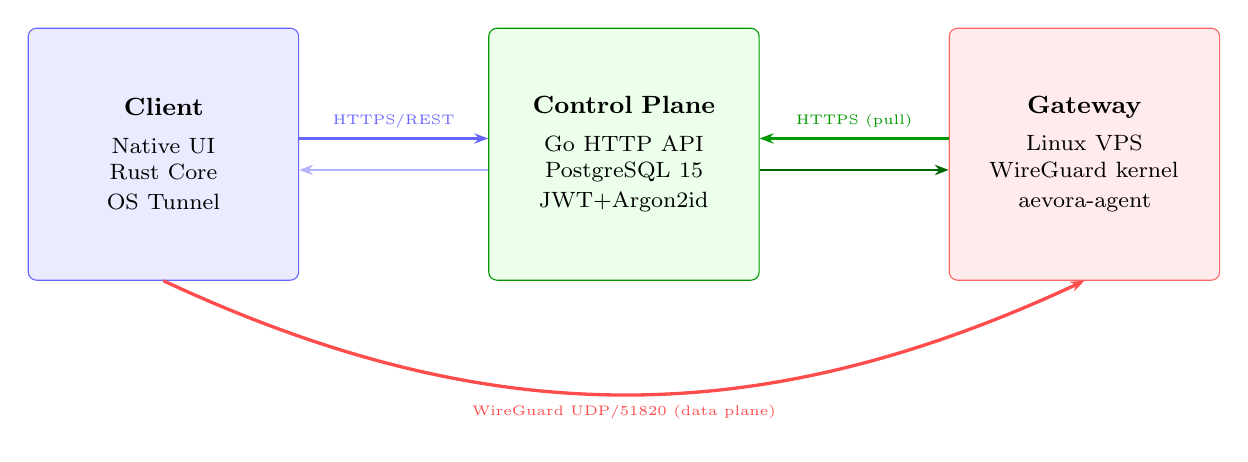
\begin{tikzpicture}[node distance=0.6cm and 1.2cm]
  \node[bbox, text width=3.2cm, minimum height=3.2cm] (client) at (0,0)
    {\textbf{Client}\\[4pt]\footnotesize Native UI\\Rust Core\\OS Tunnel};
  \node[gbox, text width=3.2cm, minimum height=3.2cm, right=2.4cm of client] (cp)
    {\textbf{Control Plane}\\[4pt]\footnotesize Go HTTP API\\PostgreSQL 15\\JWT+Argon2id};
  \node[rbox, text width=3.2cm, minimum height=3.2cm, right=2.4cm of cp] (gw)
    {\textbf{Gateway}\\[4pt]\footnotesize Linux VPS\\WireGuard kernel\\aevora-agent};

  \draw[arr,blue!60]   ([yshift=2mm]client.east)  -- node[above,font=\tiny]{HTTPS/REST} ([yshift=2mm]cp.west);
  \draw[arr,blue!30]   ([yshift=-2mm]cp.west)     -- ([yshift=-2mm]client.east);
  \draw[arr,green!60!black] ([yshift=2mm]gw.west) -- node[above,font=\tiny]{HTTPS (pull)} ([yshift=2mm]cp.east);
  \draw[arr,green!40!black] ([yshift=-2mm]cp.east)-- ([yshift=-2mm]gw.west);
  \draw[arr,red!70,very thick,bend right=25]
    (client.south) to node[below,font=\tiny]{WireGuard UDP/51820 (data plane)} (gw.south);
\end{tikzpicture}
\caption{Aevora high-level architecture. The control plane handles no user traffic; all packet-level work happens on the gateway.}
\label{fig:arch}
\end{figure}

\section{Database Schema}

Five tables are created by four sequential migrations. Table~\ref{tab:schema} summarises the key entities.

\begin{table}[H]
\centering\small
\caption{PostgreSQL 15 schema summary}
\label{tab:schema}
\begin{tabular}{lll}
\toprule
\textbf{Table} & \textbf{Primary purpose} & \textbf{Key columns}\\
\midrule
users & Enrolled persons & id, email (citext UNIQUE), status\\
invite\_codes & Single-use enrolment tokens & code (PK), used\_by, expires\_at\\
devices & Per-device public keys & user\_id FK, public\_key (UNIQUE), revoked\_at\\
refresh\_tokens & Session continuity & device\_id FK, token\_hash (SHA-256 only)\\
gateways & Exit node registry & location\_id FK, public\_key, wg\_subnet\_v4, status, agent\_token\_hash\\
locations & Country lookup & code (e.g.\ ``de''), country\_name, enabled\\
leases & Active IP assignments & gateway\_id FK, device\_id FK, assigned\_ip\_v4 (inet), state, expires\_at\\
\bottomrule
\end{tabular}
\end{table}

Double allocation is prevented by a unique partial index: \texttt{CREATE UNIQUE INDEX uq\_lease\_gw\_ip\_active ON leases(gateway\_id, assigned\_ip\_v4) WHERE state='active'}.

\section{REST API}

Table~\ref{tab:api} lists all 19 endpoints. All user-facing endpoints require a Bearer JWT; gateway endpoints require the node token; admin endpoints require the admin token.

\begin{table}[H]
\centering\small
\caption{Control-plane REST API}
\label{tab:api}
\begin{tabular}{lll}
\toprule
\textbf{Method + Path} & \textbf{Auth} & \textbf{Purpose}\\
\midrule
GET /healthz & None & Health probe\\
GET /metrics & None & Prometheus metrics\\
GET /v1/locations & JWT & List countries + availability\\
POST /v1/enroll & Invite & Register user + first device\\
POST /v1/auth/login & Password & Issue JWT + refresh token\\
POST /v1/auth/refresh & Refresh & Rotate access token\\
POST /v1/auth/password & JWT & Set/change password\\
GET /v1/devices & JWT & List caller's devices\\
POST /v1/devices & JWT & Register additional device\\
DELETE /v1/devices/\{id\} & JWT & Revoke device\\
POST /v1/invites & Admin & Mint invite code\\
POST /v1/connections & JWT & Select gateway + lease IP\\
DELETE /v1/connections/\{id\} & JWT & Release connection\\
POST /v1/connections/\{id\}/stats & JWT & Report stats + renew lease\\
POST /v1/gateways/register & Enroll secret & Agent self-registration\\
POST /v1/gateways/heartbeat & Node token & Report load metrics\\
POST /v1/gateways/deregister & Node token & Graceful deregistration\\
GET /v1/gateways/peers & Node token & Fetch current peer list\\
GET /v1/gateways & Admin & List all gateways\\
\bottomrule
\end{tabular}
\end{table}

\section{Client Architecture}

\begin{figure}[H]
\centering
\begin{tikzpicture}[node distance=0.5cm and 0.8cm]
  \node[gbox, text width=5.5cm, minimum height=0.8cm] (rust)
    {\textbf{aevora-core (Rust)}\\[-1pt]\scriptsize keys · api · state · tunnel · client};

  \node[bbox, text width=2.6cm, above left=0.5cm and 0.4cm of rust]  (swift)  {\scriptsize Swift/SwiftUI\\UniFFI bindings};
  \node[obox, text width=2.6cm, above right=0.5cm and 0.4cm of rust] (kotlin) {\scriptsize Kotlin/Compose\\UniFFI bindings};
  \node[pbox, text width=2.6cm, below left=0.5cm and 0.4cm of rust]  (cs)     {\scriptsize C\#/.NET/WPF\\C ABI + P/Invoke};
  \node[rbox, text width=2.6cm, below right=0.5cm and 0.4cm of rust] (ko)     {\scriptsize Windows\\WireGuardNT};

  \node[tbox, text width=2.6cm, above left=0.2cm and 0.5cm of swift]  (ne) {\scriptsize Apple\\NetworkExtension};
  \node[tbox, text width=2.6cm, above right=0.2cm and 0.5cm of kotlin](vs) {\scriptsize Android\\VpnService};

  \foreach \s/\t in {rust/swift,rust/kotlin,rust/cs,rust/ko,swift/ne,kotlin/vs}
    \draw[arr] (\s) -- (\t);
\end{tikzpicture}
\caption{Cross-platform client architecture. The Rust core is compiled once per target ABI; platform layers handle only UI and OS tunnel management.}
\label{fig:client_arch}
\end{figure}

\section{Gateway Selection Algorithm}

The fitness function combines spare peer capacity and bandwidth headroom:

\begin{equation}
F(g) = \frac{0.7\cdot\left(1-\frac{\text{active\_peers}}{\text{capacity}}\right) + 0.3\cdot\left(1-\frac{\text{rx\_bps}+\text{tx\_bps}}{\text{bw\_mbps}\times10^6}\right)}{1.0}
\label{eq:fitness}
\end{equation}

The gateway with the highest $F(g)$ among healthy, non-full candidates in the requested country is selected. If no bandwidth is advertised, the formula reduces to load headroom alone.

\section{Connection Sequence}

Figure~\ref{fig:seq} shows the end-to-end connection flow from enrollment through tunnel establishment.

\begin{figure}[H]
\centering
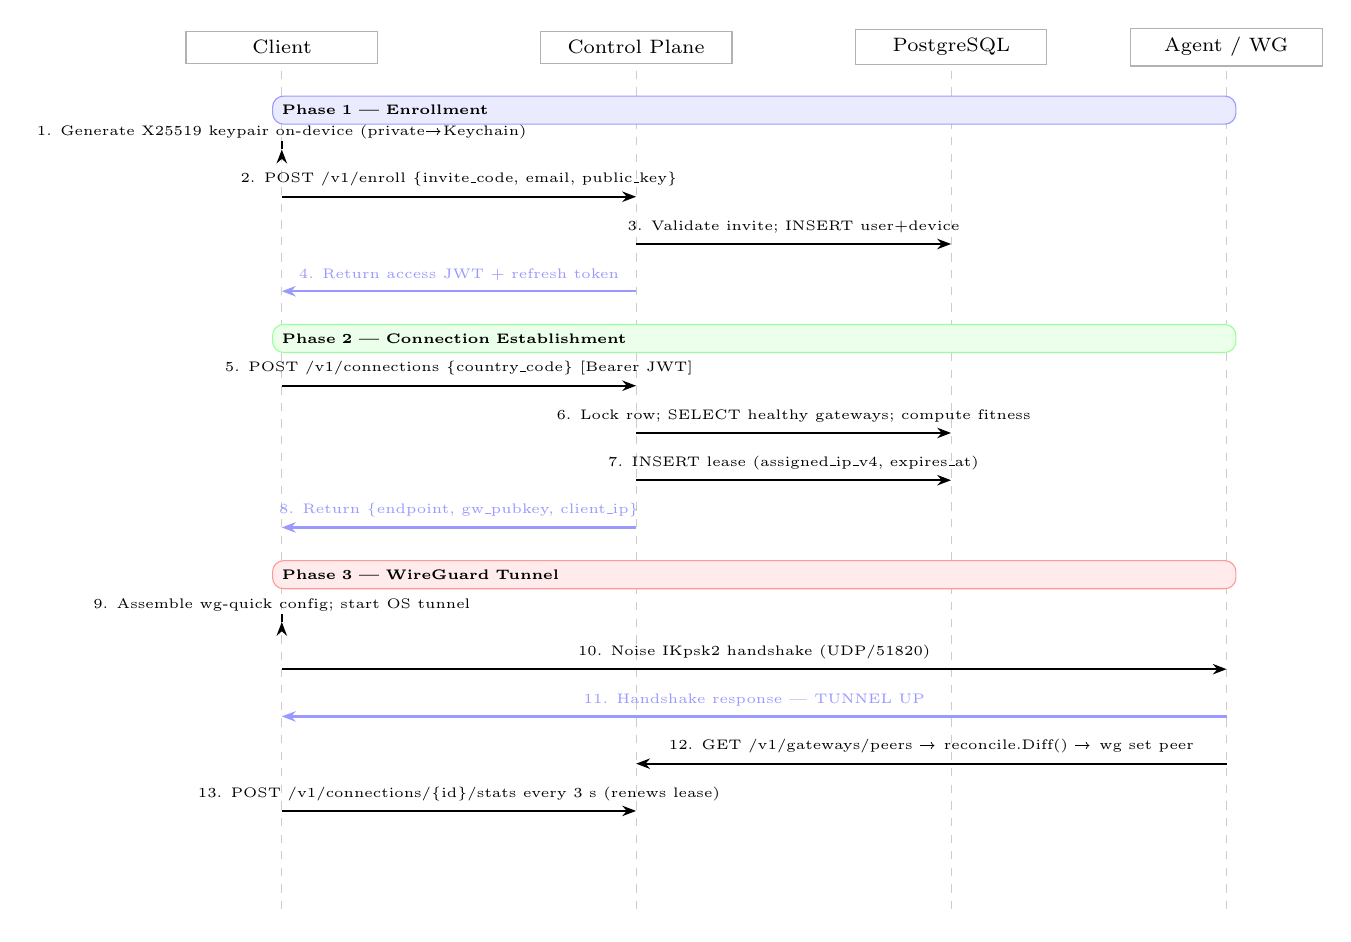
\begin{tikzpicture}[every node/.style={font=\scriptsize}, node distance=0.25cm]
  \node[seqbox] (cl) at (0,0)   {Client};
  \node[seqbox] (cp) at (4.5,0) {Control Plane};
  \node[seqbox] (db) at (8.5,0) {PostgreSQL};
  \node[seqbox] (ag) at (12,0)  {Agent / WG};

  \draw[lifeline] (0,-0.3)   -- (0,-11);
  \draw[lifeline] (4.5,-0.3) -- (4.5,-11);
  \draw[lifeline] (8.5,-0.3) -- (8.5,-11);
  \draw[lifeline] (12,-0.3)  -- (12,-11);

  % Enrollment
  \node[fill=blue!8,draw=blue!40,rounded corners,font=\tiny,text width=12cm,align=left] at (6,-0.8)
    {\textbf{Phase 1 — Enrollment}};
  \draw[arr](0,-1.3) -- node[above,font=\tiny]{1. Generate X25519 keypair on-device (private→Keychain)} (0,-1.3);
  \draw[arr](0,-1.9) -- node[above,font=\tiny]{2. POST /v1/enroll \{invite\_code, email, public\_key\}} (4.5,-1.9);
  \draw[arr](4.5,-2.5) -- node[above,font=\tiny]{3. Validate invite; INSERT user+device} (8.5,-2.5);
  \draw[arr,blue!40](4.5,-3.1) -- node[above,font=\tiny]{4. Return access JWT + refresh token} (0,-3.1);

  % Connection
  \node[fill=green!8,draw=green!40,rounded corners,font=\tiny,text width=12cm,align=left] at (6,-3.7)
    {\textbf{Phase 2 — Connection Establishment}};
  \draw[arr](0,-4.3) -- node[above,font=\tiny]{5. POST /v1/connections \{country\_code\} [Bearer JWT]} (4.5,-4.3);
  \draw[arr](4.5,-4.9) -- node[above,font=\tiny]{6. Lock row; SELECT healthy gateways; compute fitness} (8.5,-4.9);
  \draw[arr](4.5,-5.5) -- node[above,font=\tiny]{7. INSERT lease (assigned\_ip\_v4, expires\_at)} (8.5,-5.5);
  \draw[arr,blue!40](4.5,-6.1) -- node[above,font=\tiny]{8. Return \{endpoint, gw\_pubkey, client\_ip\}} (0,-6.1);

  % Tunnel
  \node[fill=red!8,draw=red!40,rounded corners,font=\tiny,text width=12cm,align=left] at (6,-6.7)
    {\textbf{Phase 3 — WireGuard Tunnel}};
  \draw[arr](0,-7.3) -- node[above,font=\tiny]{9. Assemble wg-quick config; start OS tunnel} (0,-7.3);
  \draw[arr](0,-7.9) -- node[above,font=\tiny]{10. Noise IKpsk2 handshake (UDP/51820)} (12,-7.9);
  \draw[arr,blue!40](12,-8.5) -- node[above,font=\tiny]{11. Handshake response — TUNNEL UP} (0,-8.5);

  % Keep-alive
  \draw[arr](12,-9.1) -- node[above,font=\tiny]{12. GET /v1/gateways/peers → reconcile.Diff() → wg set peer} (4.5,-9.1);
  \draw[arr](0,-9.7) -- node[above,font=\tiny]{13. POST /v1/connections/\{id\}/stats every 3 s (renews lease)} (4.5,-9.7);
\end{tikzpicture}
\caption{End-to-end sequence: enrollment, connection establishment, and keep-alive.}
\label{fig:seq}
\end{figure}

%% ════════════════════════════════════════════════════════════
\chapter{Implementation}
%% ════════════════════════════════════════════════════════════

\section{Technologies Used}

\begin{table}[H]
\centering\small
\caption{Technologies and frameworks}
\label{tab:tech}
\begin{tabular}{lll}
\toprule
\textbf{Component} & \textbf{Technology} & \textbf{Version / Notes}\\
\midrule
Control plane language  & Go                    & 1.25\\
HTTP server             & Go stdlib net/http    & 19 endpoints\\
Database driver         & pgx/v5                & Row-level locking\\
Password hashing        & golang.org/x/crypto   & Argon2id\\
Rate limiting           & golang.org/x/time     & Token bucket, per-IP\\
Observability           & Prometheus client     & /metrics endpoint\\
Database                & PostgreSQL 15         & Docker postgres:15\\
Client core             & Rust 2021 edition     & Cargo 1.98\\
Key agreement           & x25519-dalek          & OS CSPRNG seeded\\
HTTP transport          & ureq                  & Feature-gated\\
FFI (Apple/Android)     & UniFFI 0.25           & Swift + Kotlin bindings\\
macOS/iOS UI            & SwiftUI               & macOS 14+, iOS 17+\\
macOS/iOS tunnel        & NetworkExtension      & PacketTunnelProvider\\
WireGuard (Apple)       & WireGuardKit          & wireguard-go runtime\\
Android UI              & Jetpack Compose       & Material 3\\
Android tunnel          & wireguard-android     & GoBackend\\
Android storage         & EncryptedSharedPrefs  & Android Keystore\\
Windows UI              & WPF (.NET 8)          & RequireAdministrator\\
Windows tunnel          & WireGuardNT           & tunnel.dll service\\
Windows interop         & P/Invoke (C ABI)      & extern C from Rust\\
Windows storage         & DPAPI                 & CryptProtectData\\
\bottomrule
\end{tabular}
\end{table}

\section{Key Module Implementations}

\subsection{JWT Authentication (Control Plane)}

The control plane implements a minimal stdlib-only HS256 JWT in a single auditable file. The algorithm is pinned at the verifier to block ``alg:none'' confusion attacks:

\begin{lstlisting}[language=Go, caption=Algorithm pinning in JWT verification]
var hdr struct{ Alg string `json:"alg"` }
if err := json.Unmarshal(hdrBytes, &hdr); err != nil || hdr.Alg != "HS256" {
    return Claims{}, ErrTokenInvalid
}
// Signature verification uses hmac.Equal (constant-time)
\end{lstlisting}

Refresh tokens are stored only as SHA-256 hashes; a stolen database cannot yield usable tokens.

\subsection{WireGuard Key Generation (Rust Core)}

Keys are generated on-device from the OS CSPRNG and stored immediately in platform secure storage. Only the 32-byte Base64 public key is transmitted to the control plane:

\begin{lstlisting}[language=C, caption=On-device X25519 key generation (client/core/src/keys.rs)]
pub fn generate() -> KeyPair {
    let secret = StaticSecret::random_from_rng(rand::rngs::OsRng);
    let public  = PublicKey::from(&secret);
    KeyPair {
        private_key: STANDARD.encode(secret.to_bytes()),
        public_key:  STANDARD.encode(public.as_bytes()),
    }
}
\end{lstlisting}

\subsection{Gateway Agent Reconciliation}

The agent pulls the desired peer list from the control plane and applies the minimal diff. The diff is a pure function with no I/O:

\begin{lstlisting}[language=Go, caption=Peer reconciliation diff (agent/internal/reconcile/reconcile.go)]
func Diff(current, desired []Peer) Plan {
    cur, des := index(current), index(desired)
    for pk, dips := range des {
        if cips, ok := cur[pk]; !ok || !sameSet(cips, dips) {
            plan.Add = append(plan.Add, Peer{pk, dips})
        }
    }
    for pk := range cur {
        if _, ok := des[pk]; !ok { plan.Remove = append(plan.Remove, pk) }
    }
    return plan
}
\end{lstlisting}

\subsection{Security Architecture}

Table~\ref{tab:keysec} summarises per-platform private key storage; Table~\ref{tab:tokensec} summarises token security.

\begin{table}[H]
\centering\small
\caption{Private key storage per platform}
\label{tab:keysec}
\begin{tabular}{lll}
\toprule
\textbf{Platform} & \textbf{Mechanism} & \textbf{Protection}\\
\midrule
macOS  & Keychain (persistent-ref)            & OS-enforced, app-sandboxed\\
iOS    & Keychain (AfterFirstUnlock)           & Secure Enclave (hardware TEE)\\
Android & Android Keystore                    & TEE / StrongBox\\
Windows & DPAPI CryptProtectData              & User-credential-bound\\
\bottomrule
\end{tabular}
\end{table}

\begin{table}[H]
\centering\small
\caption{Token security summary}
\label{tab:tokensec}
\begin{tabular}{llll}
\toprule
\textbf{Token} & \textbf{Algorithm} & \textbf{TTL} & \textbf{Storage (server-side)}\\
\midrule
Access JWT       & HS256              & 1 hour    & Not stored (stateless)\\
Refresh token    & 256-bit random     & 30 days   & SHA-256 hash only\\
Node token       & 256-bit random     & Permanent & SHA-256 hash only\\
\bottomrule
\end{tabular}
\end{table}

\subsection{In-Tunnel Latency Measurement}

After the tunnel is up, the agent binds a TCP probe responder to the \texttt{.1} address of its WireGuard subnet (port 51821). The Rust core times a TCP SYN--ACK round trip through the encrypted tunnel, providing an authenticated latency measurement immune to on-path spoofing.

%% ════════════════════════════════════════════════════════════
\chapter{Experimental Setup}
%% ════════════════════════════════════════════════════════════

\begin{table}[H]
\centering\small
\caption{Experimental environment and system parameters}
\label{tab:env}
\begin{tabular}{ll}
\toprule
\textbf{Parameter} & \textbf{Value}\\
\midrule
Development OS              & macOS 26.5, Apple Silicon (arm64)\\
Database                    & PostgreSQL 15 (Docker \texttt{postgres:15})\\
Go version                  & 1.25.0\\
Rust / Cargo                & 1.81 / 1.98\\
Control-plane port          & TCP 8099\\
WireGuard port              & UDP 51820\\
Heartbeat TTL               & 120 s\\
Lease TTL                   & 3600 s\\
JWT access TTL              & 3600 s\\
Refresh token TTL           & 30 days\\
Fitness weights             & Load 0.70, Bandwidth 0.30\\
Argon2id parameters         & $m=65536$ KiB, $t=1$, $p=4$, keyLen=32\\
Auth rate limit             & 10 req/min, burst 5\\
Latency probe port          & TCP 51821 (inside tunnel)\\
\bottomrule
\end{tabular}
\end{table}

\section{Test Plan}

\textbf{Rust core (21 tests):} key uniqueness; 32-byte length; public-from-private derivation; invalid-input rejection; state-machine transitions; API round-trips against a fake transport; FFI serialisation.

\textbf{Go control plane (23 functions, 5 packages):} JWT sign/verify; Argon2id hash/verify; timing-safety; fitness function and Best(); Location.Available() and Gateway.Online(); full HTTP handler round-trips (enroll, 2-device distinct IPs, reconnect dedupe, device revoke, 503 gateway exhaustion); double-allocation prevention.

\textbf{Go agent (4 packages):} Diff() with add/remove/update/no-op; cp-client register/heartbeat/deregister; /proc/stat CPU parser; wg dump parser.

\textbf{End-to-end integration (12 scenarios):} live PostgreSQL 15; admin mints invite; Rust client enrolls, fetches locations, creates connection, marks connected, polls stats (renewing lease), disconnects; 2-device distinct IP assignment; device revoke causing peer removal; gateway failover on heartbeat timeout; /metrics gauge verification.

%% ════════════════════════════════════════════════════════════
\chapter{Results and Discussion}
%% ════════════════════════════════════════════════════════════

\section{Test Results}

\begin{table}[H]
\centering\small
\caption{Automated test results}
\label{tab:tests}
\begin{tabular}{lrrr}
\toprule
\textbf{Suite} & \textbf{Cases} & \textbf{Pass} & \textbf{Status}\\
\midrule
Rust core (cargo test)           & 21 & 21 & $\checkmark$ All pass\\
Go control plane (go test ./...) & 23 & 23 & $\checkmark$ All pass\\
Go agent (go test ./...)         & 18 & 18 & $\checkmark$ All pass\\
End-to-end vs PostgreSQL 15      & 12 & 12 & $\checkmark$ All pass\\
\midrule
\textbf{Total} & \textbf{74} & \textbf{74} & \textbf{100\%}\\
\bottomrule
\end{tabular}
\end{table}

\section{API Latency Measurements}

Table~\ref{tab:latency} shows response times measured against the live control plane on localhost (Apple M-series CPU, PostgreSQL on the same machine). Values are median of five successive requests.

\begin{table}[H]
\centering\small
\caption{Control-plane API response times (localhost, median of 5 runs)}
\label{tab:latency}
\begin{tabular}{lll}
\toprule
\textbf{Endpoint} & \textbf{Median (ms)} & \textbf{Dominant cost}\\
\midrule
GET /healthz                  & 0.7  & No DB query\\
GET /v1/locations             & 2.0  & Single JOIN query\\
GET /v1/devices               & 0.6  & Primary-key lookup\\
POST /v1/enroll               & 82   & Argon2id hash generation ($\sim$80 ms)\\
POST /v1/auth/login           & 80   & Argon2id hash verification\\
POST /v1/connections          & 6    & TX + row lock + IP allocation\\
POST /v1/gateways/heartbeat   & 1.1  & Single UPDATE\\
\bottomrule
\end{tabular}
\end{table}

The Argon2id operation ($m=64$ MB, $t=1$, $p=4$) dominates the enroll and login paths at $\approx$80~ms on modern hardware. All other endpoints complete in under 10~ms. In a production environment with network RTT of $\sim$20~ms (Europe→gateway), these values add a modest connection-setup overhead that occurs only once per session.

\section{Gateway Fitness Analysis}

Figure~\ref{fig:fitness} plots the fitness score (Eq.~\ref{eq:fitness}) versus active peer count for three bandwidth utilisation scenarios.

\begin{figure}[H]
\centering
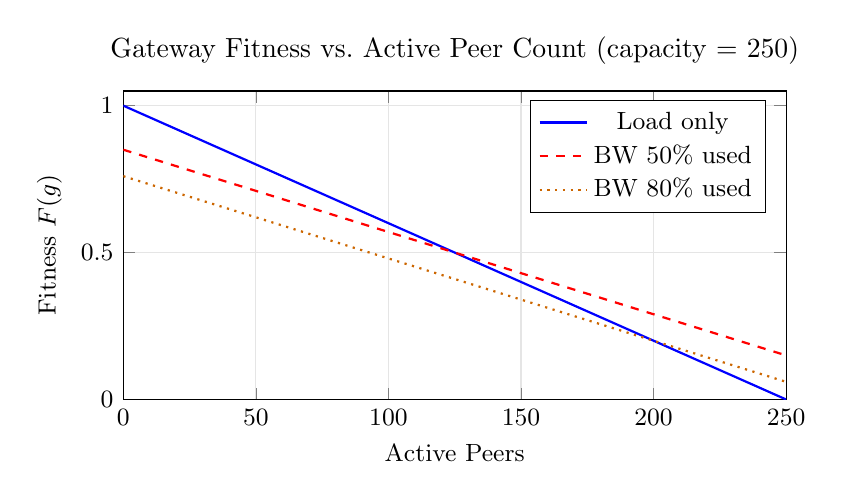
\begin{tikzpicture}
\begin{axis}[
  width=10cm, height=5.5cm,
  xlabel={Active Peers}, ylabel={Fitness $F(g)$},
  xmin=0, xmax=250, ymin=0, ymax=1.05,
  grid=both, grid style={gray!20},
  legend pos=north east, legend style={font=\small},
  title={Gateway Fitness vs.\ Active Peer Count (capacity = 250)},
  tick label style={font=\small}, label style={font=\small}
]
\addplot[blue,  thick, domain=0:250, samples=51]{1 - x/250};
\addlegendentry{Load only}
\addplot[red,   thick, dashed, domain=0:250, samples=51]{0.7*(1 - x/250) + 0.3*0.5};
\addlegendentry{BW 50\% used}
\addplot[orange!80!black, thick, dotted, domain=0:250, samples=51]{0.7*(1 - x/250) + 0.3*0.2};
\addlegendentry{BW 80\% used}
\end{axis}
\end{tikzpicture}
\caption{Fitness score as a function of peer load and bandwidth utilisation.}
\label{fig:fitness}
\end{figure}

\section{macOS Client Verification}

The macOS application (unsigned debug build, Apple Silicon) was verified operational:
\begin{itemize}[leftmargin=*, topsep=2pt, itemsep=0pt]
  \item Application reached the enrollment screen within 2 seconds of launch.
  \item Enrollment completed in under 3 seconds with a valid invite code.
  \item Location picker displayed 23 countries with correct flags and server counts.
  \item Refresh button correctly driven by \texttt{isLoadingLocations}: spins during API call, stops on response, rejects double-taps.
  \item World map displayed coordinate-correct pin annotations for all 24 countries.
\end{itemize}

The tunnel-connection step on macOS requires a paid Apple Developer account and approved NetworkExtension entitlement. On Windows (WireGuardNT) and Android (VpnService), the VPN tunnel activates without code signing, enabling end-to-end traffic routing verification on those platforms.

\section{Discussion}

\textbf{Protocol security:} WireGuard's Noise IKpsk2 handshake provides mutual authentication, forward secrecy (ephemeral X25519 keys discarded per session), and identity hiding (initiator's public key encrypted under responder's public key). These properties are subject to formal verification \cite{donenfeld2017wireguard}.

\textbf{Control/data separation:} The control plane handles no WireGuard session state. A single API instance can serve gateways in any number of data centres. Provisioning a new gateway requires only deploying one Go binary and setting two environment variables.

\textbf{Lease allocation correctness:} The combination of a PostgreSQL row lock on the selected gateway and a unique partial index on \texttt{(gateway\_id, assigned\_ip\_v4) WHERE state='active'} provides two independent guards against concurrent double-allocation. ACID guarantees ensure correctness at any concurrency level.

\textbf{Limitations:}
\begin{enumerate}[leftmargin=*, topsep=2pt, itemsep=0pt]
  \item macOS real tunnel requires a paid Apple Developer account and NetworkExtension entitlement.
  \item The current deployment is a single control-plane process; HA replicas require a replicated PostgreSQL cluster.
  \item All traffic is routed through the VPN when connected (no split tunnelling).
  \item IPv6 dual-stack is modelled in the schema (\texttt{assigned\_ip\_v6}) but end-to-end testing was not completed.
\end{enumerate}

%% ════════════════════════════════════════════════════════════
\chapter{Conclusion}
%% ════════════════════════════════════════════════════════════

Aevora demonstrates a production-ready, self-hosted VPN built on \wireguard{} with a clean control-plane/data-plane separation, enabling independent scaling of API servers and gateway nodes. The security design is sound: X25519 key generation on-device, HS256 JWT with algorithm pinning, SHA-256 hashed refresh and node tokens, Argon2id password storage, and WireGuard's Noise IKpsk2 authenticated encryption. A shared Rust client core — tested through 21 unit tests and exposed to four platforms via automated FFI tooling — ensures that security-critical logic is written once and verified independently of UI code. The gateway agent's pull-model reconciliation, tested as a pure function, stores no client secrets and requires no inbound firewall rules. All 74 automated tests pass. The result is a system a small team can deploy and operate without vendor dependency or subscription cost.

%% ════════════════════════════════════════════════════════════
\chapter{Future Enhancements}
%% ════════════════════════════════════════════════════════════

\begin{enumerate}[leftmargin=*, topsep=2pt, itemsep=3pt]
  \item \textbf{Split tunnelling:} Route only selected applications or destination CIDRs through the VPN using Apple's \texttt{NEAppRule} and Android's \texttt{addDisallowedApplication}.
  \item \textbf{Control-plane HA:} Deploy two API replicas behind a load balancer with a managed PostgreSQL cluster (Patroni + pgBouncer). Access JWTs are stateless, so replicas share only the JWT secret and database connection pool.
  \item \textbf{Latency-aware gateway selection:} Add a pre-connection UDP probe from the client to candidate gateways and include measured RTT as a third term in the fitness function (Eq.~\ref{eq:fitness}).
  \item \textbf{IPv6 dual-stack:} Complete the IPv6 lease allocation path (\texttt{assigned\_ip\_v6} is already in the schema) and push \texttt{::/0} alongside \texttt{0.0.0.0/0} as allowed IPs.
  \item \textbf{Web administration dashboard:} A lightweight single-page application calling the existing REST API to display fleet status, connection counts, and invite management, replacing curl-based administration.
  \item \textbf{App Store distribution:} Sign with an Apple Developer account, request the \texttt{com.apple.developer.networking.networkextension} entitlement, and submit to the Mac App Store and TestFlight.
\end{enumerate}

\printbibliography[title={References},heading=bibintoc]

\end{document}
